\section{ESMF Superstructure:  Coupling and Control}
\label{sec:superclasses}

\subsection{Introduction}

In this section, we describe the classes involved in the ESMF superstructure, 
their relationships, and typical action sequences for component interactions.

\subsection{Design Goals and Considerations}

One of the primary goals of the ESMF project is to increase interoperability
across a range of Earth system modeling components.  Initially these 
components will be large scale, such as land models, ocean models, 
and data assimilation systems.  Earth system research 
often requires that such components be coupled together in multiple
configurations.  We identify user-supplied components discretized on grids with 
a {\tt Gridded Component} class, and the software used to couple them together
with a {\tt Coupler Component} class.  

As the framework evolves, we plan to utilize ESMF coupling services for 
smaller-scale tasks within model components, such as the transformation of 
data between the 
physics and dynamics in a spectral atmospheric model, and the creation 
of nested higher resolution regions within a coarser grid.  The goal is 
to couple components at varying scales both flexibly and efficiently.  
Our strategies for accomplishing this are as follows.

We aim to keep the coupling specification entirely external 
to {\tt Gridded Component}s involved in an interaction, which makes it easier 
for the same {\tt Gridded Component} to be reconfigured for a different 
coupled application.
This is closely related to the ``mediator'' strategy for handling complexity in 
software that requires many inter-component interactions (see Section~\ref{sec:oop}).  
We avoid excessive complication in the {\tt Coupler Component} by limiting
its responsibility; the {\tt Coupler} component does not instantiate 
interacting components, schedule, or run them.  These tasks are performed
by an {\tt Application Component} or other parent component (see 
Section~\ref{sec:controlflow}).

The ability to remap to adapt to different computing platform sizes 
and characteristics is essential for performance portability.
Where their physics content permits
{\tt Gridded Component}s can be configured for
sequential or concurrent execution without changes to the {\tt Gridded 
Component} code.  Changes to {\tt Coupler} and/or {\tt Application Component} code are likely to 
be required (see Section~\ref{sec:scoping}). This is possible because 
the {\tt Gridded Component} uses the infrastructure layer to abstract communication
protocols such that a {\tt Gridded Component} looks the same on all
platforms. Additionally, the superstructure layer ensures that a {\tt Gridded
Component} can be created to execute concurrently or sequentially through the
manipulation of PE lists.

The ability to overlap computation with communication is also essential for
performance.  We facilitate this by enabling the user to initiate data 
sends during {\tt Gridded Component} execution, as soon as the data is ready.

To further increase efficiency, data may be sent between components without 
needing to be sent to a {\tt Coupler} as an intermediate step (see
Section~\ref{sec:dataflow}).

It is not necessary to create return points from 
within the time iteration loop of a {\tt Gridded Component}.  This reduces the
amount of work application groups will need to perform to adopt the 
framework.

There is considerable interest in evolving the ESMF into a more comprehensive
Problem Solving Environment (PSE).  The systematized approach to component 
scheduling we have adopted will enable a layer of tools for application 
configuration to be added to the architecture in the future.

\subsection{Classes and Scoping}
\label{sec:scoping}
There are restrictions on how ESMF components within an Earth system application 
can be scoped on a parallel platform.  There is only one {\tt Application Component} 
defined for any application; it initially allocates resources and tracks 
application-wide information. 
The {\tt Application Component} must be instantiated on 
any {\tt Decomposition Elements}\footnote{In ESMF {\tt Decomposition Elements} are the
basic abstraction that provides platform neutral parallelism, they are discussed in detail
in Section~\ref{sec:progmodel}} or {\tt DE}s on 
which other components
within the application are defined.  This is true whether the 
application consists of a single executable or multiple 
executables.  

An ESMF coupled application typically involves an {\tt Application Component} 
containing two or more {\tt Gridded Component}s that require an 
inter-component data exchange, and one or more {\tt Coupler 
Component}s.  However, any parent component that contains the appropriate 
subcomponents can manage their execution and coupling.  ESMF thereby
supports applications consisting of a hierarchy of coupled systems.

A {\tt Coupler Component} must be instantiated on any {\tt DE}s on which components
it will couple are defined.  This is consistent with an architectural
model in which communication is handled internal to components, and all
inter-component interactions are local (see Section~\ref{sec:strategies}).  
It is possible for
some portions of the functionality of a component to be restricted to
a subset of the {\tt DE}s over which the component is defined.  For example, 
it may be computationally efficient for the computation of interpolation
weights to occur on a set of {\tt DE}s not being used by any {\tt Gridded 
Components}
in the application.  The {\tt Coupler} might define a subcomponent on 
those {\tt DE}s specifically to handle the interpolation function.

A {\tt Gridded Component} may exist across all {\tt DE}s in an {\tt Application}.  
When a set of {\tt Gridded  Component}s and a {\tt Coupler} all execute in sequence on 
the same set of {\tt DE}s and are contained within an application running 
as a single executable we have a sequential execution SPMD configuration.  

Within an application, a {\tt Gridded Component} may also reside on 
a subset of {\tt DE}s.  These {\tt DE}s may wholly coincide with, be wholly 
contained within or wholly contain another component.  

It is possible for ESMF applications to contain some component sets
that are executing sequentially and others that are executing concurrently.
We might have, for example, atmosphere and land components instantiated 
on the same set of 
{\tt DE}s and running as one executable, ocean and sea ice 
components instantiated on a separate set of {\tt DE}s and running as 
another executable, and a {\tt Coupler} and {\tt Application Component} 
instantiated across all {\tt DE}s.

Figure~\ref{fig:couplerscaling} illustrates scoping of components
in a coupled, hierarchically structured application.  At the top level, 
a climate application consists of atmosphere and ocean components 
instantiated on mutually exclusive {\tt DE} sets.  These components communicate 
via an atmosphere/ocean {\tt Coupler} defined on the union of their {\tt DE}s.  
Scheduling is controlled by an {\tt Application
Component} which is also defined across all {\tt DE}s.  The atmosphere component
is similarly structured as a coupled application.  It consists of a 
physics component and a dynamics component, which are both distributed
across all the atmospheric {\tt DE}s.  A physics/dynamics {\tt Coupler} controls
the data transpose between these subcomponents.  In this case, the
atmospheric component rather than the highest level application component
controls the coupling sequence.  

\begin{figure}
\caption[{Scoping of Components in a Coupled Application}]{A coupled
application may itself be composed of other coupled systems.}
\label{fig:couplerscaling}
\begin{center}
\scalebox{0.7}{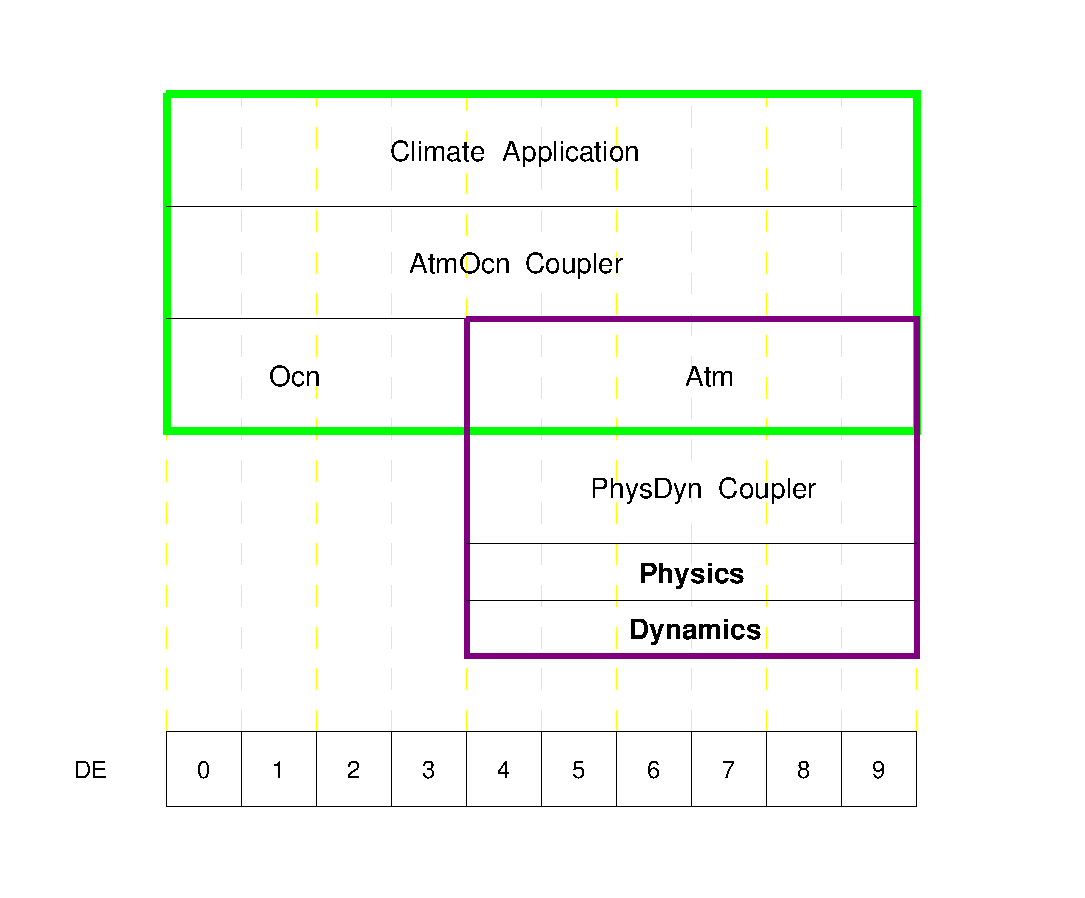
\includegraphics{CouplerScaling.eps}}
\end{center}
\end{figure}


\subsection{Flow of Control}
\label{sec:controlflow}
{\tt Gridded components} have few responsibilities with respect to coupling
to other components.  They do not need to keep track of the data needed
by other components or to provide methods for inter-component 
grid transformations or transfers of data.  They {\it are} responsible for 
providing a description of all of the fields and data they
can export to other components, and for similarly providing a description 
of the data they require in order to run.  These descriptions are
embodied in the {\tt ESMF\_State} class, and the kind of data that they 
represent is identified by the {\tt type} attribute of that class, which can
have an {\tt ESMF\_IMPORT} or {\tt ESMF\_EXPORT} value.  The {\tt State} class
includes metadata information, actual pointers to data 
locations, and default criteria for data validation.  The last of these in its
simplest form may be a bit that is set when data is ready for use.  The ESMF 
will provide methods that enable a user to add or remove fields and data from 
{\tt State}s.  

A {\tt Coupler Component} produces a specification of the sequence of 
operations that are necessary to effect communication between components, 
both scientific and computational, generic and user-defined.  The {\tt Coupler} 
returns these to the {\tt Application} or parent in the form of a set of {\tt Transform} objects 
along with associated sequencing restrictions.  Each {\tt Transform} has a
function pointer to a transform operation and may be bundled with 
associated data, information about coupling frequency, and 
data validation criteria.

The {\tt Application} or parent component initiates the coupling and manages 
its scheduling.  It is responsible for instantiating the {\tt Gridded Component}s
that are exchanging data and instantiating the {\tt Coupler}, for setting up the desired 
sequencing, and making the calls to the methods of the components and 
{\tt Coupler} that effect the exchange.  The parent may partition the 
transforms
for execution among the {\tt Gridded Component}s and the {\tt Coupler}, so that, for 
example, a data send or coupling transformation can occur while a {\tt Gridded 
Component} is executing, without a need for the component to return to the
parent level.  
To disable or rearrange the coupling sequence, a different set of function
pointers can be passed to the component.

The {\tt ESMF\_StateTransform} call executes a {\tt Transform} 
within a {\tt Gridded Component}.  It takes as arguments a
{\tt Transform} object and the component's import or export {\tt State}.  
For {\tt Transform}s that initiate non-blocking sends, a {\tt ESMF\_StateTransformComplete} 
call can check that data  buffers are available for reuse.  This 
call takes the initiated {\tt Transform} object as an argument.

The {\tt ESMF\_StateValidate} call evaluates whether a component's 
import {\tt State} is ready for use.  It may check the entire {\tt State} or 
a specified subset.

\subsection{Flow of Data}
\label{sec:dataflow}
The design choices we have made enable the user to configure ESMF
applications so that data is transferred from one component to another, 
without requiring that it first be sent via message passing to a
{\tt Coupler} (or even necessarily
copied).  This is likely to be the most efficient way of performing 
inter-component coupling when the components are instantiated on different
{\tt DE} sets.  However, if desired, an application can also be configured so that
data from a source component is sent to a distinct set of {\tt Coupler} 
{\tt DE}s for processing before being sent to its destination.

\section{Examples}

Here we describe a number of example scenarios of ESMF usage. The examples are
described in text and illustrated using UML sequence diagrams. In these diagrams
The vertical axis is time, positive
downward, and the horizontal axis shows the objects that are involved in the
exchange.  Arrowed lines to text boxes mean that the source of the arrow has
created the object in the box.  Solid lines to the start of a vertical
box indicate a method call.  Dashed lines indicate a return.
The overall flow of execution is partitioned into four stages in this
discussion, {\it Create Sequence}, {\it Configure Sequence}, {\it Run Sequence}
and {\it Termination Sequence}.
 
\subsection{Create Sequences}

An ESMF application begins with the creation of components. The
three sequence diagrams in figures \ref{fig:ApplicationComponentCreate}, 
\ref{fig:CouplerComponentCreate} and 
\ref{fig:GriddedComponentCreate} show the
component creations steps for different types of component.


\subsubsection{Application Creation}
Figure \ref{fig:ApplicationComponentCreate} shows the sequence associated with
creation of components from an {\tt Application Component}. In the diagram,
creation of child components executes concurrently. The application component
proceeds through three phases which are serialized with respect to one another.
First the application component creates a registry object for this application,
next it creates two gridded components, finally it creates two coupler
components for transporting and translating data between gridded components.
The actions within each phase can be parallelized, however, the phases
themselves execute sequentially.
\begin{figure}
\caption[{Application Component Create}]
{The UML sequence for application component creation}
\label{fig:ApplicationComponentCreate}
\scalebox{1.0}{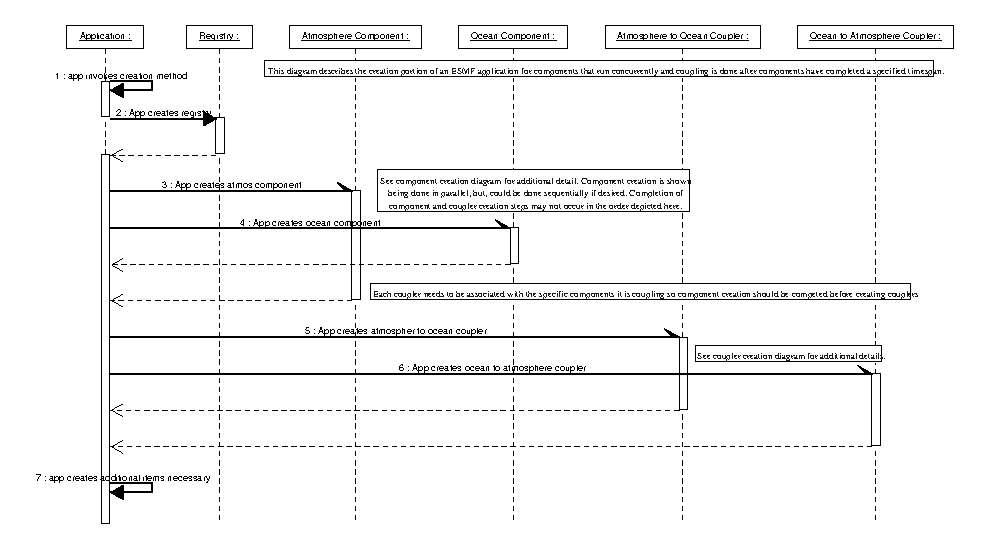
\includegraphics{CreateAppDiagram.eps}}
\end{figure}

\subsubsection{Coupler Component Creation}
Figure \ref{fig:CouplerComponentCreate} shows the sequence associated
with creation in a {\tt Coupler Component}. The key steps involved are
the creation of import and export states that respectively hold inputs and
outputs of the coupler component. Coupler component creation may also involve
internal, coupler component specific initialization and, additionally,
registering the coupler components presence with the global registry entity.

\begin{figure}
\caption[{Coupler Component Create}]
{The UML sequence for coupler component creation}
\begin{center}
\label{fig:CouplerComponentCreate}
\scalebox{1.0}{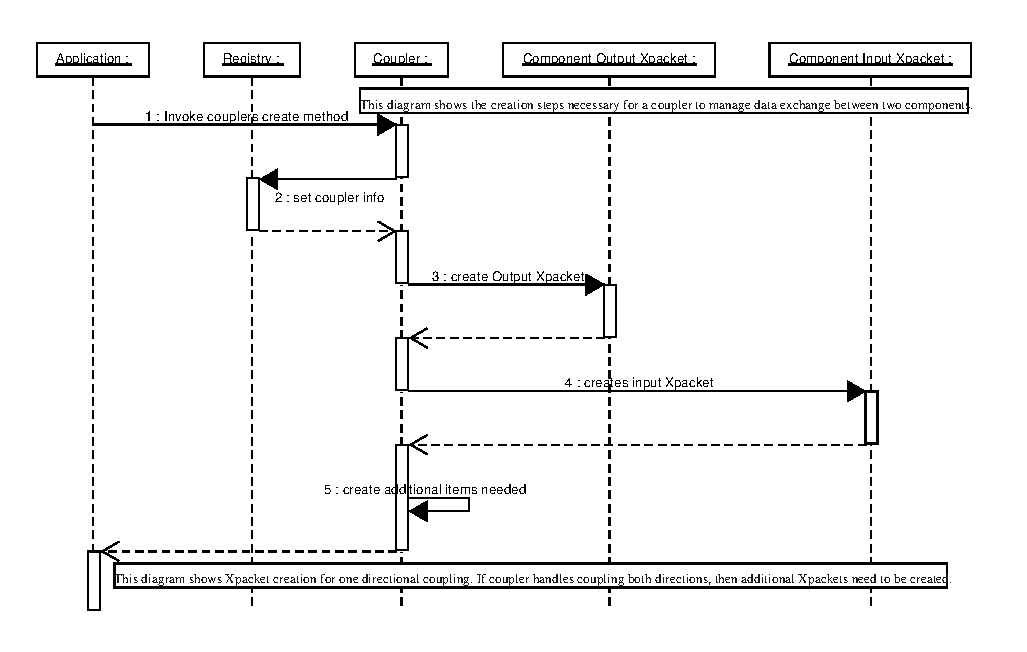
\includegraphics{CreateCouplerDiagram.eps}}
\end{center}
\end{figure}

\subsubsection{Gridded Component Creation}
Figure \ref{fig:GriddedComponentCreate} shows the sequence associated with
creation in a {\tt Gridded Component}. A key step in Gridded Component
creation is the creation of import and export states for transferring 
data to and from other components. In addition there may be component
specific computation that is executed during creation as well as execution
of a registration function to register the component in the global registry.

\begin{figure}
\caption[{Gridded Component Create}]
{The UML sequence for gridded component creation}
\begin{center}
\label{fig:GriddedComponentCreate}
\scalebox{1.0}{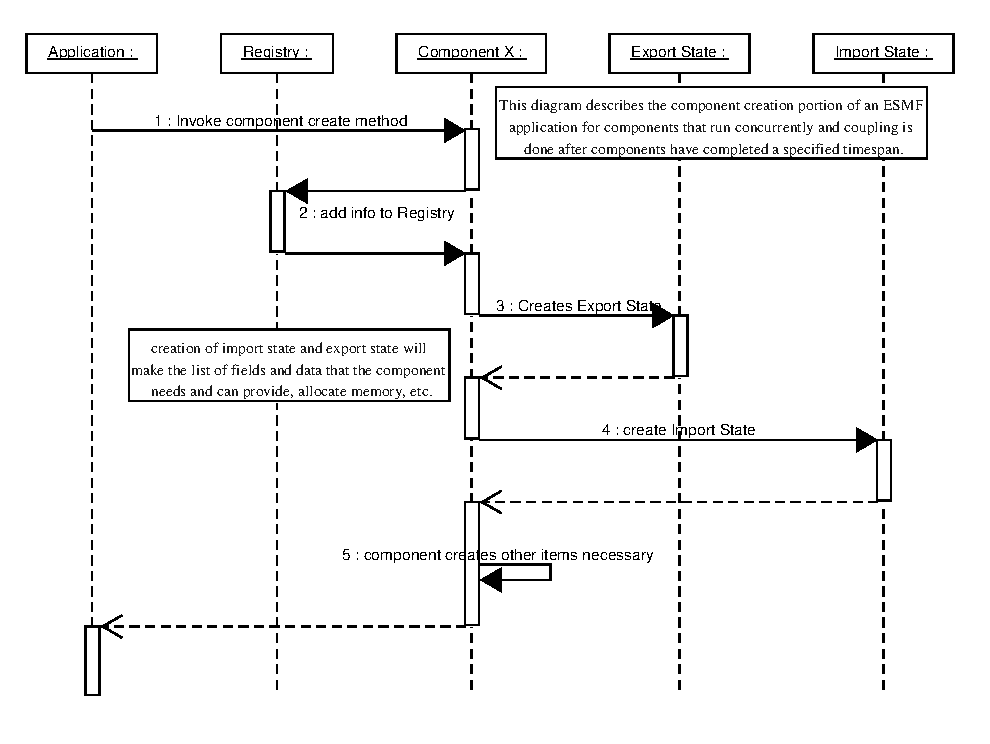
\includegraphics{CreateComponentDiagram.eps}}
\end{center}
\end{figure}

\subsection{Configure Sequences}
Following component creation a configuration step is invoked. This step
invokes component specific logic that is responsible for setting the component
initial state. Figures \ref{fig:ApplicationComponentConfigure}, 
\ref{fig:CouplerComponentConfigure} and 
\ref{fig:GriddedComponentConfigure} show the component
configuration sequences for different types of component.

\subsubsection{Application Component Configuration}
Figure \ref{fig:ApplicationComponentConfigure} shows the sequence associated 
with configuration in an {\tt Application Component}. The sequence begins 
with internal configuration of the application component. The application
component then invokes the configuration methods for the gridded components
within its scope and for the coupler components within its scope.
Gridded component configuration completes before coupler component
configuration in invoked. In the example shown in the figure configuration
for the individual gridded components executes concurrently as does 
configuration for the individual coupler components.


\begin{figure}
\caption[{Application Component Configuration}]
{The UML sequence for application component configuration}
\begin{center}
\label{fig:ApplicationComponentConfigure}
\scalebox{1.0}{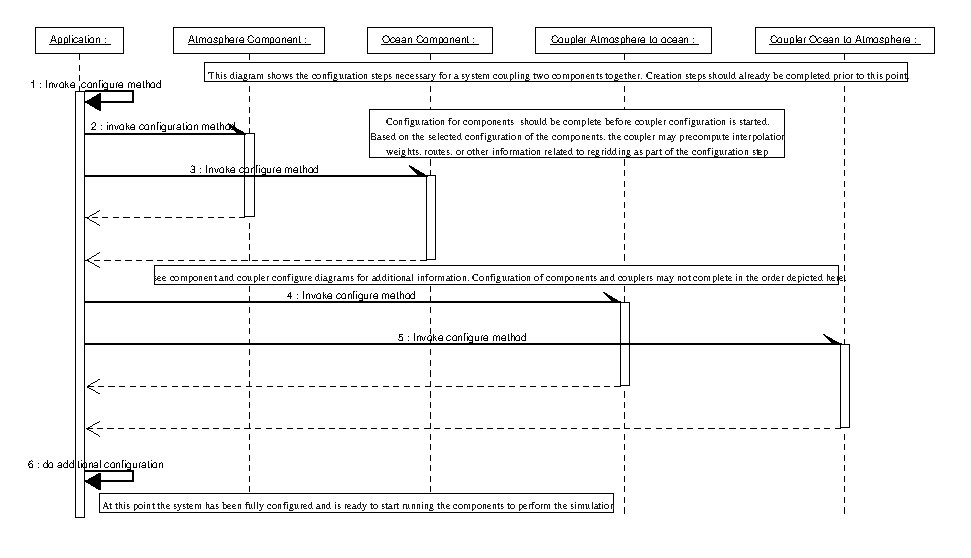
\includegraphics{ConfigureAppDiagram.eps}}
\end{center}
\end{figure}

\subsubsection{Coupler Component Configuration}
Figure \ref{fig:CouplerComponentConfigure} shows the sequence associated 
with configuration of a {\tt Coupler Component}. A coupler components
configuration method is invoked from its parent
component (the {\tt Application Component} in the case of
figure \ref{fig:CouplerComponentConfigure}). Once invoked the method
is responsible for initializing the coupler's import and export states 
to a known, valid condition. Additional computation, specific to a particular
coupler component, may also be included. This could include precalculation
of interpolation weights that are repeatedly used in a specific regridding
operation.

\begin{figure}
\caption[{Coupler Component Configuration}]
{The UML sequence for coupler component configuration}
\begin{center}
\label{fig:CouplerComponentConfigure}
\scalebox{1.0}{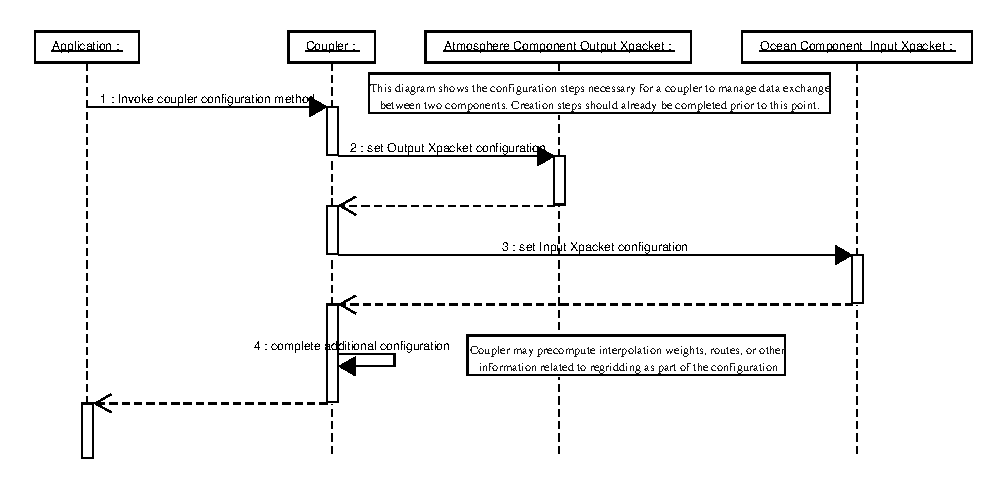
\includegraphics{ConfigureCouplerDiagram.eps}}
\end{center}
\end{figure}

\subsubsection{Gridded Component Configuration}
Figure \ref{fig:GriddedComponentConfigure} shows the sequence associated 
with configuration in a {\tt Gridded Component}. The component configuration
method is invoked from the parent component (the {\tt Application Component}
in figure \ref{fig:GriddedComponentConfigure}). Once invoked the configuration
stage is responsible for configuring the import and export states for the 
component to a known, valid status. Component configuration may also include
specialized configuration steps specific to that particular
component. On completion the configuration method returns to the
parent component.

\begin{figure}
\caption[{Gridded Component Configuration}]
{The UML sequence for gridded component configuration}
\begin{center}
\label{fig:GriddedComponentConfigure}
\scalebox{1.0}{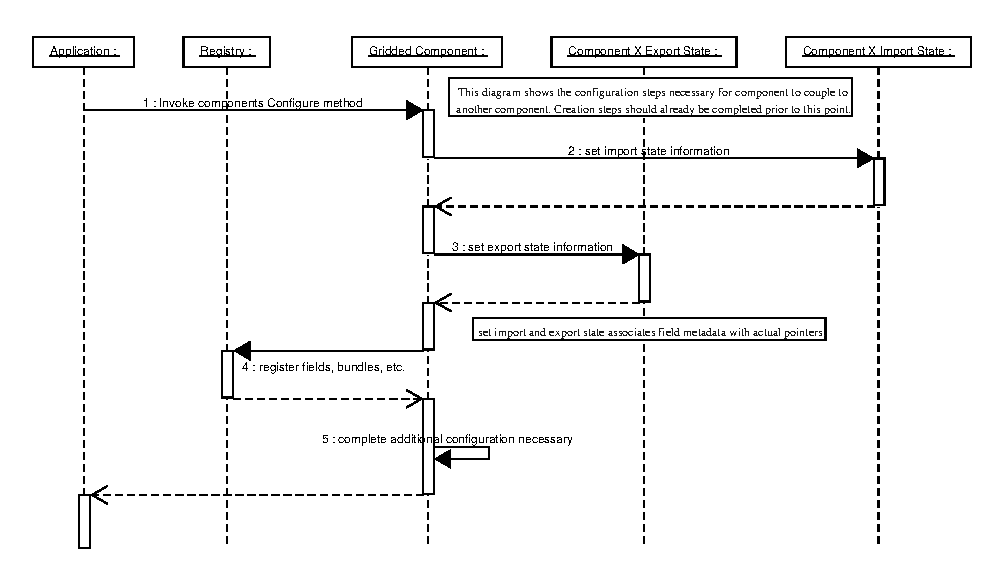
\includegraphics{ConfigureComponentDiagram.eps}}
\end{center}
\end{figure}

\subsection{Run sequences}
This section shows sequence diagrams for a number of different run scenarios.
For each sequence, the preceding component creation and component configuration 
phases are omitted for clarity.

\subsubsection{Concurrent coupled atmosphere ocean sequence}

Figure \ref{fig:RunApplicationDiagram} shows the sequence of actions involved
in running an atmosphere ocean coupled system. In the example the
coupling is two-way, with the ocean receiving data from the atmosphere and 
sending data back to the atmosphere.  Atmosphere and ocean components are 
configured for concurrent execution.

\begin{figure}
\caption[{Basic Run Application}]{A prototypical UML sequence for a basic Run Application stage.\\}
\label{fig:RunApplicationDiagram}
\scalebox{1.0}{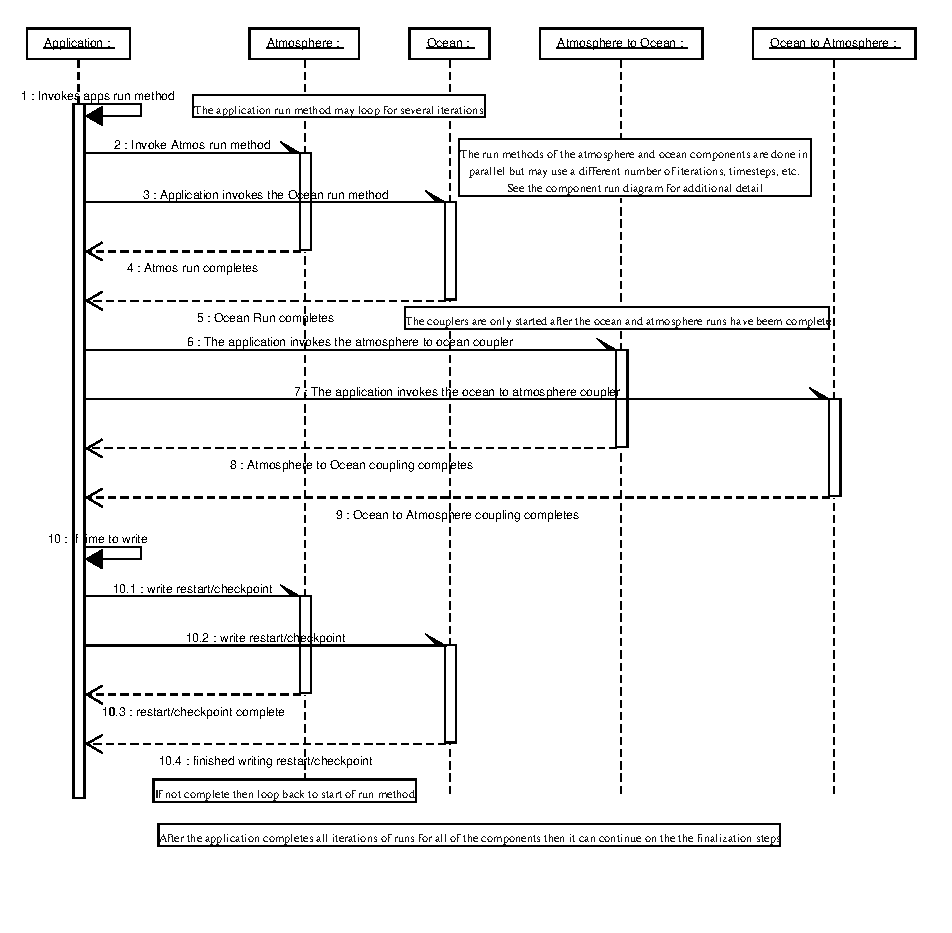
\includegraphics{runApplicationDiagram.eps}}
\end{figure}

Following {\tt Application Component} startup (and coupler and component
creation and configuration) the run methods of components are 
invoked. An example of this procedure is illustrated in figure 
\ref{fig:RunApplicationDiagram}. In 
the example given, the {\tt Application Component} invokes the run method of 
the of the Atmosphere and Ocean gridded components concurrently. The 
application 
component then waits until these stages are complete before it invokes the 
coupler components run methods. The coupler components
take export states from the atmosphere and ocean respectively. 
The coupler components are invoked to run concurrently with one another. Before iterating 
onto the next time step the {\tt Application Component} selectively invokes the 
checkpoint/restart methods of the Ocean and Atmosphere components, again 
concurrently. Finally the {\tt Application Component} evaluates whether
to exit or whether to return to the start of the run loop for subsequent 
iteration.

\subsubsection{Sequential Components Run Sequence}

Figure \ref{fig:SequentialComponentsRunSequence} shows the UML sequence
for a multi-component application in which components execute serially
with respect to one another. Each component may itself be a parallel
computation, however, execution of methods in one component do not overlap 
with execution of methods in other component in this example.
For an individual object the event sequence mirrors the procedure in 
figure \ref{fig:RunApplicationDiagram}. However, in the sequential
case only one event is active at any time.
\begin{figure}
\caption[{Sequential Component Run}]{Sequence for serial multi-component
application.\\}
\begin{center}
\label{fig:SequentialComponentsRunSequence}
\scalebox{1.0}{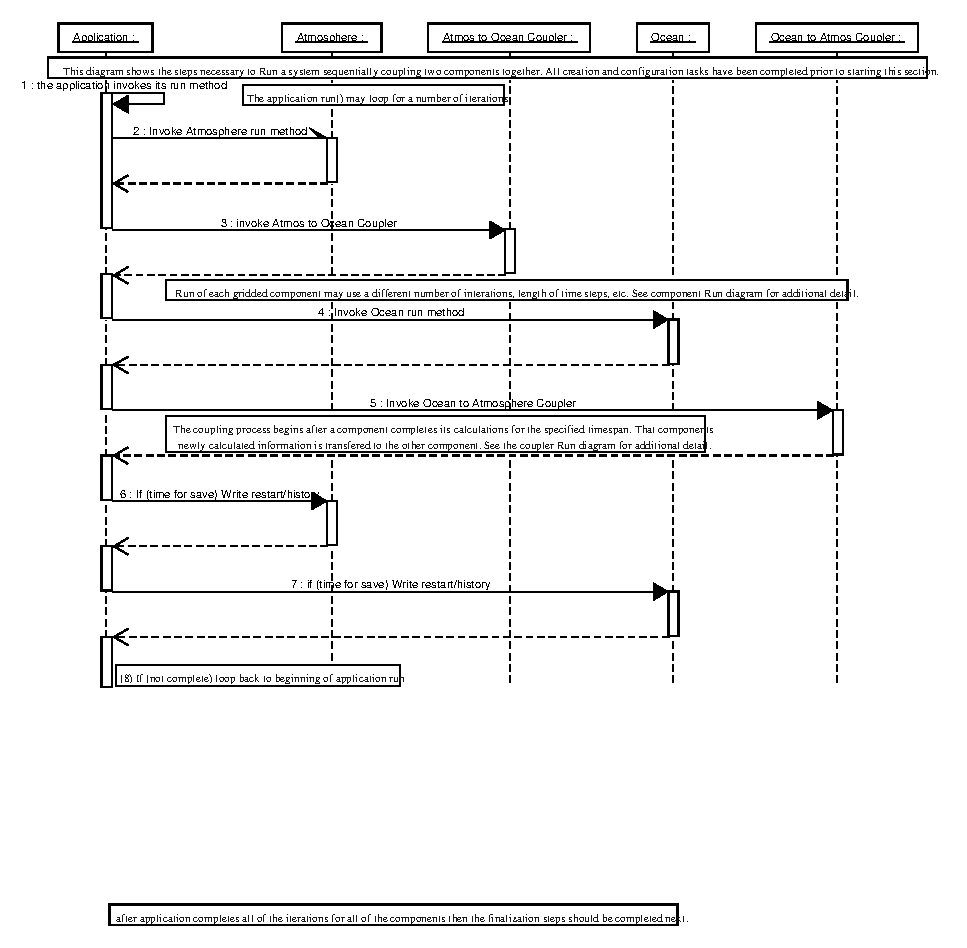
\includegraphics{RunAppSequencialDiagram.eps}}
\end{center}
\end{figure}

\subsubsection{Subcomponent Run Sequence}
Figure \ref{fig:SubcomponentRunSequence} shows the execution of an
application with components and subcomponents. In this case the 
two components (atmospheric physics and atmospheric dynamics) are 
subcomponents
of a parent atmosphere component. This configuration requires that extra 
coupler components be employed. These map between import and export states of 
the physics and dynamics components within the the scope of the
parent atmosphere component. In this scenario the sequencing of
subcomponents is controlled by their parent (the atmosphere component)
and not by the application component.

\begin{figure}
\caption[{Subcomponent Run}]{Sequence for component and subcomponent
application.\\}
\begin{center}
\label{fig:SubcomponentRunSequence}
\scalebox{1.0}{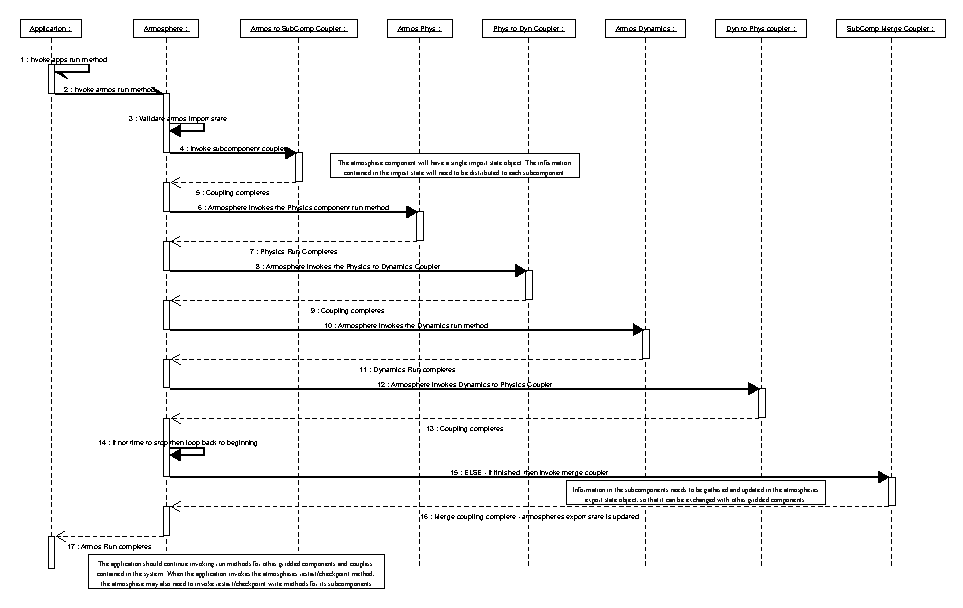
\includegraphics{subcomponentCoupling.eps}}
\end{center}
\end{figure}

\subsubsection{Ensemble Run Sequence}
Figure \ref{fig:EnsembleComponentsRunSequence} shows an ensemble scenario
in which multiple instances of the same component execute in parallel.
The run sequence is driven from the application component. However,
an extra level of coupling indirection is required. This is provided by a
coupler component that merges (in some user defined manner) the export
state of multiple ocean components. The output from this coupler
component is then passed to a coupler component that transforms from an
ocean export state to an
atmosphere component import state.
\begin{figure}
\caption[{Ensemble component Run}]{Sequence for ensemble components
application scenario.\\}
\begin{center}
\label{fig:EnsembleComponentsRunSequence}
\scalebox{1.0}{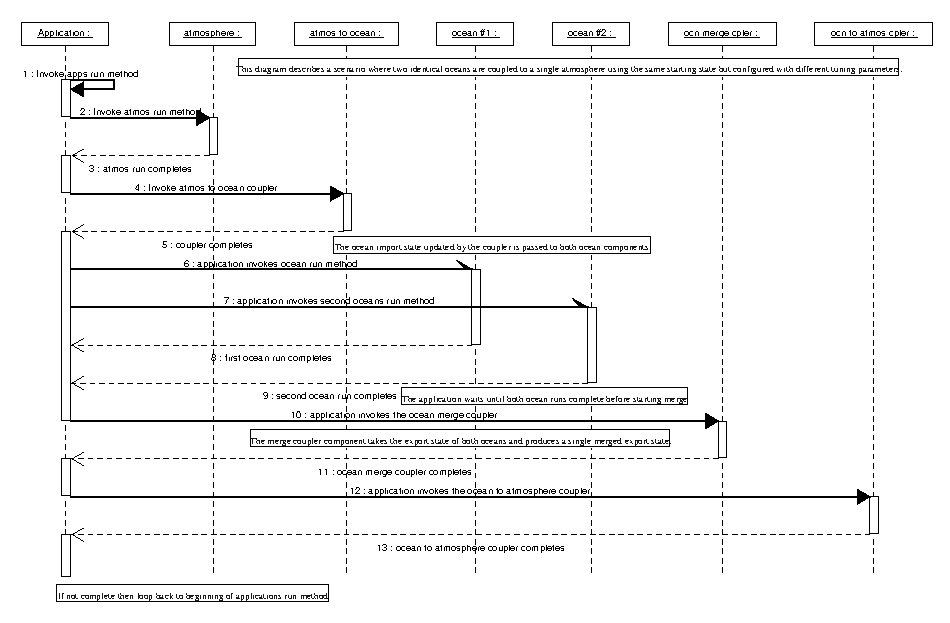
\includegraphics{runMergedApplicationDiagrams.eps}}
\end{center}
\end{figure}

\subsubsection{Ensemble Coupler Component Run Sequence}
Figure \ref{fig:EnsembleComponentsCouplerRunSequence} shows the
{\tt Coupler Component} run sequence in an ensemble scenario. The sequencing
illustrated is invoked from the application component. It proceeds by
first merging two ocean import states into a composite form. The composite
form then serves to update a merged ocean export state that is
configured for import into an ocean-to-atmosphere coupler component 
(labeled {\tt ocn to atmos cpler:} in the figure).
\begin{figure}
\caption[{Ensemble Coupler Run}]{Sequence for ensemble coupler
scenario.\\}
\begin{center}
\label{fig:EnsembleComponentsCouplerRunSequence}
\scalebox{1.0}{\includegraphics{runMergedCouplerDiagram.eps}}
\end{center}
\end{figure}

\subsubsection{Gridded Component Run Sequence}
Figure \ref{fig:GriddedComponentsRunSequence} shows the internal sequence
that a typical gridded component run method executes. This sequence, 
executed when the components run method is invoked,
consists of decoding and parsing the import state, ''stepping forward'' the 
components internal state, and setting an appropriate export state. The 
component then returns to the parent level.
\begin{figure}
\caption[{Sequence in a Component Run}]{Sequence for a component
run stage.\\}
\begin{center}
\label{fig:GriddedComponentsRunSequence}
\scalebox{1.0}{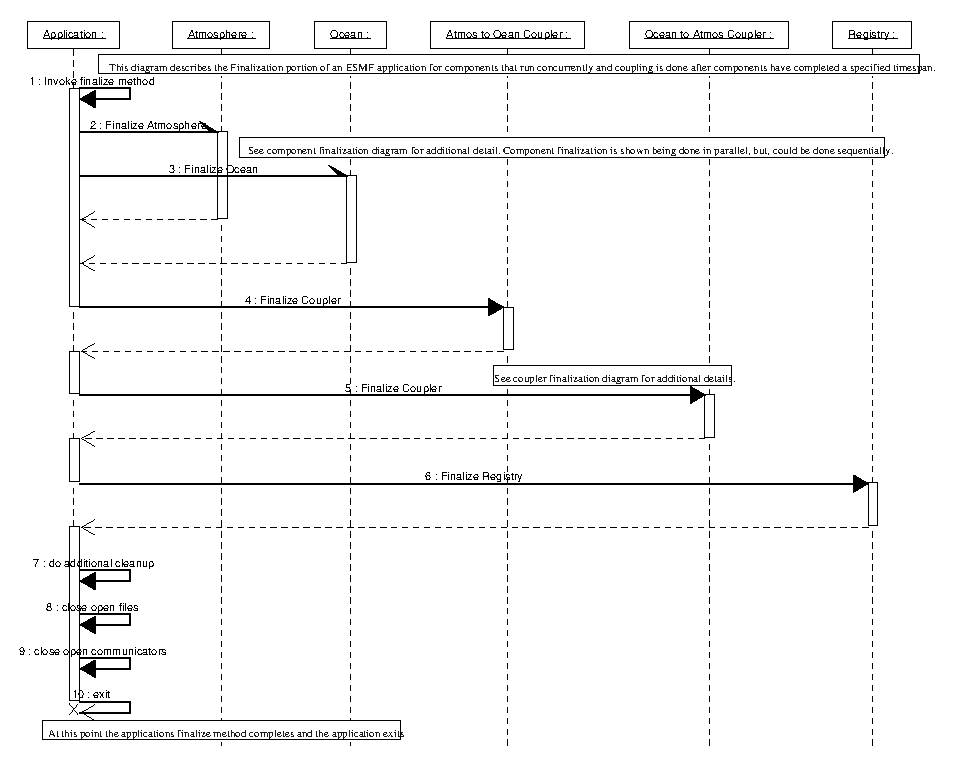
\includegraphics{RunComponentDiagram.eps}}
\end{center}
\end{figure}

\subsubsection{Coupler Component Run Sequence}
Figure \ref{fig:CouplerComponentsRunSequence} shows the internal sequence
that a typical coupler component run method executes. After invocation
from the parent level, this sequence consists
of acquiring, decoding and parsing the export state from another component.
The state is then transformed through regridding and other conversion
procedures. The transformed state is then posted as the import state
for another component and flow returns to the parent component.
\begin{figure}
\caption[{Coupler Component Run Sequence}]{Sequence for a coupler component
run stage.\\}
\begin{center}
\label{fig:CouplerComponentsRunSequence}
\scalebox{1.0}{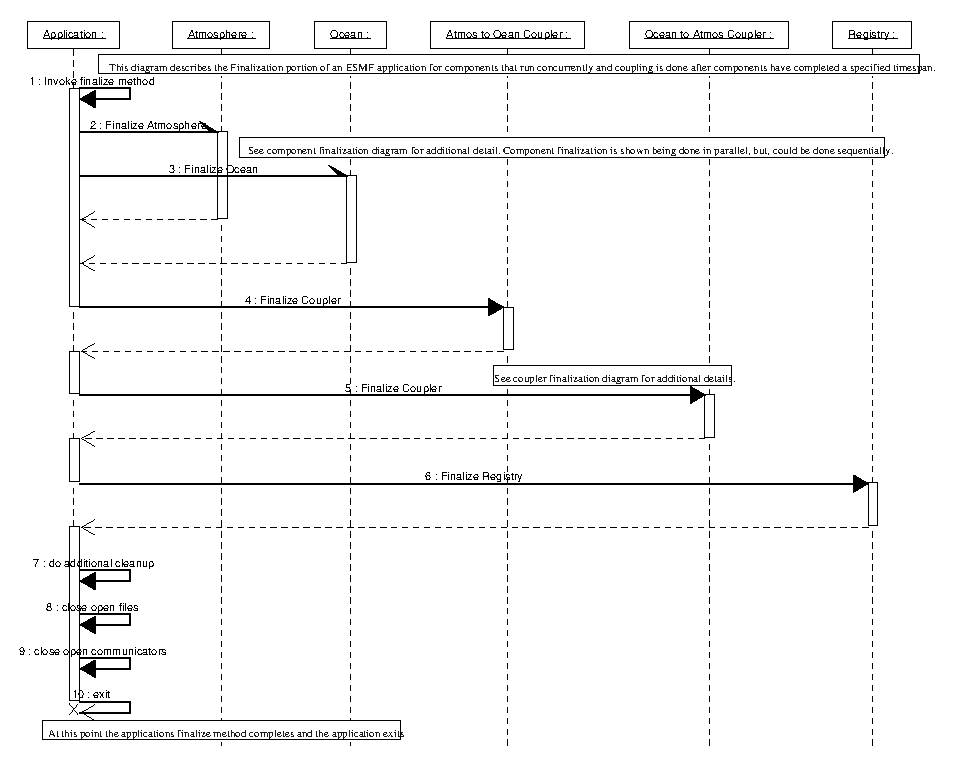
\includegraphics{RunCouplerDiagram.eps}}
\end{center}
\end{figure}

\subsection{Finalize Sequence}
Shut down of an ESMF application follows a regular sequence for each component
type. Figures 
\ref{fig:ApplicationFinalizeSequence}, 
\ref{fig:CouplerFinalizeSequence} and 
\ref{fig:GriddedComponentFinalizeSequence} show the shut down sequence for 
{\tt Application Components}, {\tt Coupler Components} and {\tt Gridded Components} respectively.
\subsubsection{Application Finalize Sequence}

Figure \ref{fig:ApplicationFinalizeSequence} shows the termination sequence
for an {\tt Application Component}. This sequence is executed at
the end of an ESMF application. The sequence consists of an invocation
of the application destroy method which then invokes the destruction methods 
of all the application component's child components. After the child 
components are destroyed the registry object and any other high-level 
structures are also destroyed.

\begin{figure}
\caption[{Application Finalize}]{Sequence for finalizing an application
component.\\}
\begin{center}
\label{fig:ApplicationFinalizeSequence}
\scalebox{1.0}{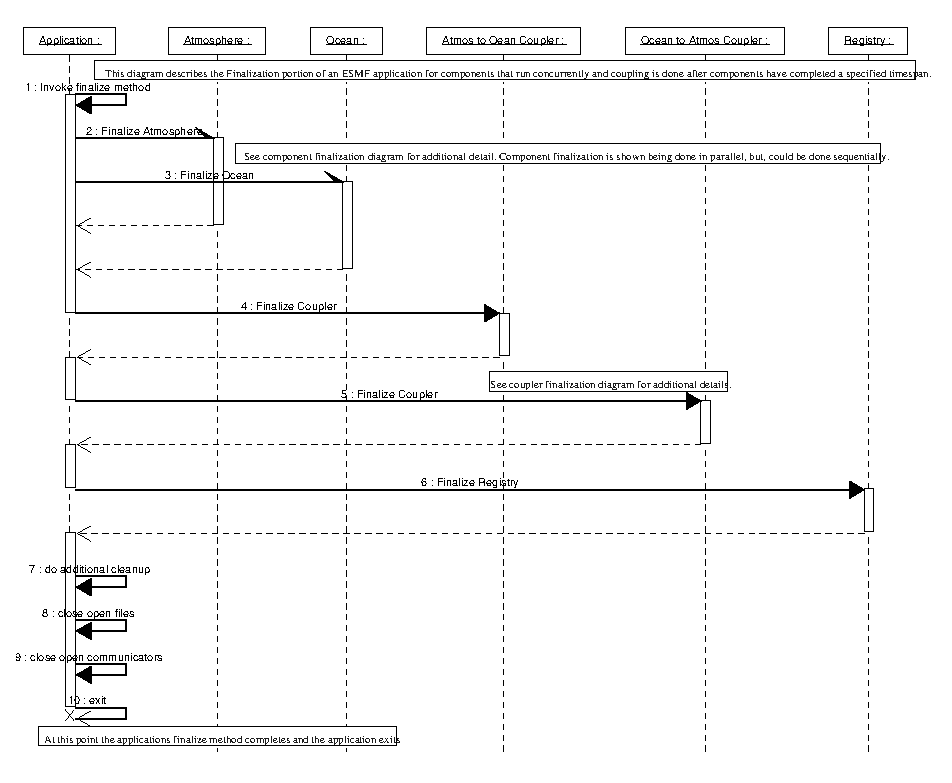
\includegraphics{FinalizeAppDiagram.eps}}
\end{center}
\end{figure}

\subsubsection{Coupler Finalize Sequence}
Figure \ref{fig:CouplerFinalizeSequence} shows the termination sequence in
a {\tt  Coupler Component}. The sequence is initiated by the parent 
component (in this example the {\tt Application Component}). Upon 
initiation a {\tt Coupler Component} destroy method will delete
the import and export state objects it instantiated at creation and
also perform file and network I/O cleanup operations.
Flow then returns to the parent component.
\begin{figure}
\caption[{Coupler Finalize}]{Sequence for finalizing a coupler component}
\begin{center}
\label{fig:CouplerFinalizeSequence}
\scalebox{1.0}{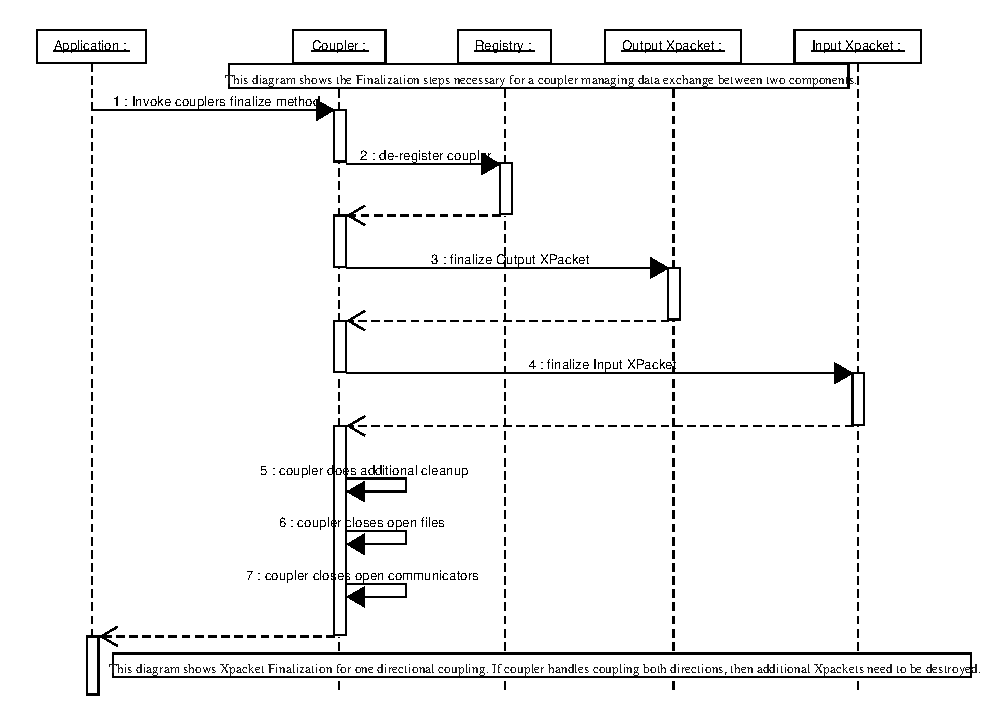
\includegraphics{FinalizeCouplerDiagram.eps}}
\end{center}
\end{figure}

\subsubsection{Gridded Component Finalize Sequence}
Figure \ref{fig:GriddedComponentFinalizeSequence} shows the termination 
sequence in a {\tt Gridded Component}. After being invoked from the
its parent component a gridded component finalize method destroys
export state and import state objects it created along with any
internal structures it has created. Then file and network I/O objects
are closed. Finally flow returns to the parent component.
\begin{figure}
\caption[{Gridded Component Finalize}]{Sequence for finalizing a gridded component}
\begin{center}
\label{fig:GriddedComponentFinalizeSequence}
\scalebox{1.0}{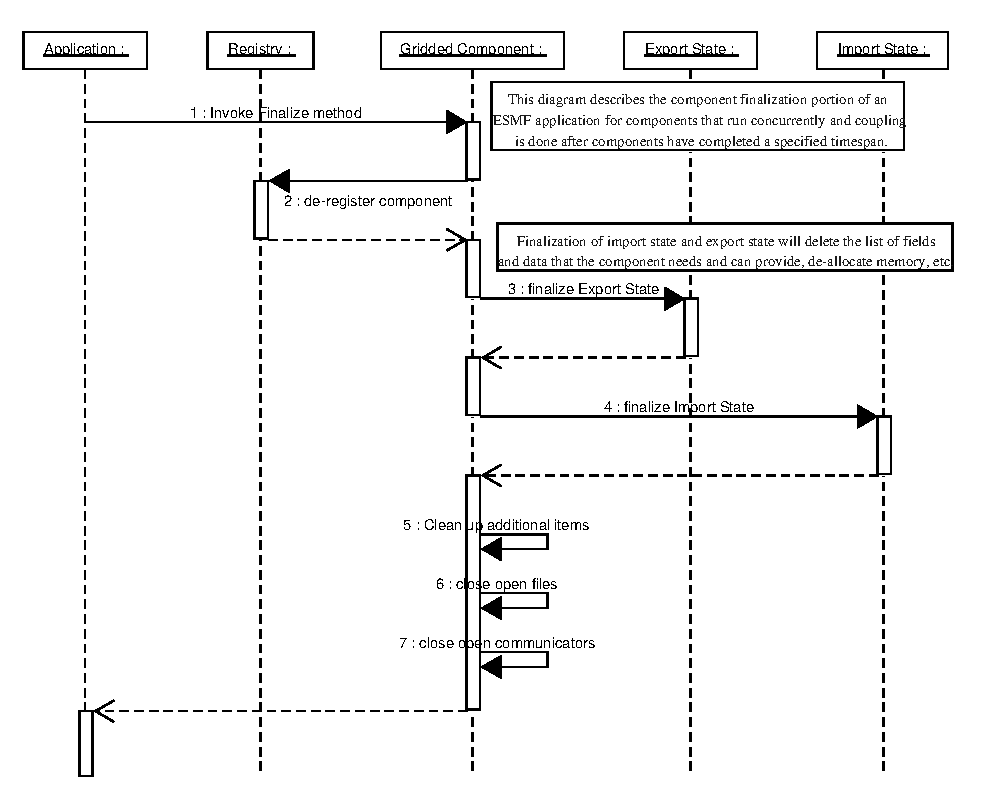
\includegraphics{FinalizeComponentDiagram.eps}}
\end{center}
\end{figure}

\section{Superstructure Class Descriptions}

The following are brief descriptions of the objects involved in the
ESMF superstructure. The relationship between the key component classes
({\tt Application Component}, {\tt Gridded Component}, {\tt Coupler Component} and the generic ESMF Component)
is shown in the 
class diagram figure \ref{fig:ESMFComponentDiagram}, which shows the relationships between these component 
types within an application. More detailed descriptions of each class 
in the ESMF superstructure layer can be found in individual class documentation.

\begin{figure}
\caption[{Component Classes}]{The relationship between basic component categories in ESMF.} 
\label{fig:ESMFComponentDiagram}
\scalebox{0.70}{\includegraphics{ESMFComponentDiagram.eps}}
\end{figure}

\subsection{Component (ESMF\_Comp)} 
A {\tt Component} is a functionally related computational entity that 
represents a large system.  The {\tt Component} base class defines a set of operations and
attributes common to all {\tt Component}s.  These include methods such as:
initialize, run, finalize, get distribution, get processor list, get status, 
and retrieve information about subcomponents.  
All {\tt Coupler}s, {\tt Gridded Component}s and {\tt Application}s possess 
these methods. 

\subsection{Application Component }

The {\tt Application Component} class is responsible for managing those 
functions that relate to an entire scientific application running under ESMF.
The {\tt Application} initialize method 
must be called at the start of any user application operating under the framework, and
the finalize method at its end.  At initialization the {\tt Application} allocates and 
configures any resources needed to run the framework.  The {\tt Application}
class can be queried for information such as an experiment name, model name, and run 
type (ESMF\_INIT, ESMF\_BRANCH, etc.).  

\subsection{Coupler Component }
A {\tt Coupler} is a user-customized type of {\tt Component} that 
encompasses all the functionality needed to communicate data between two or 
more {\tt Component}s.  A {\tt Coupler} has a coupling initiation method that 
defines and returns a set of {\tt Transform}s. In general, a {\tt Coupler Component} does not instantiate, schedule or run components whose purpose is unrelated 
to coupling, although it may mediate data exchanges among such components.
However, any component may instantiate subcomponents. It is possible
for a {\tt Coupler Component} to instantiate a subcomponent to handle a
specific part of the coupling functionality, such as calculating fluxes
or interpolation weights.


\subsection{Gridded Component }
\label{sec:griddedcomponent} 
A {\tt Gridded Component} is a user-customized {\tt Component} 
that typically represents a physical system discretized on some spatial grid.
The {\tt Gridded Component} class has methods for writing 
fields and data to an import and export {\tt State}, for verifying that
these states are fully or partially complete, and for returning these
states when queried.

\subsection{State (ESMF\_State)}
A {\tt State} is a description of a set of data that a 
{\tt Gridded Component} either needs to run or can make available.  
{\tt State}s
have a {\tt type} attribute that can have values of {\tt ESMF\_IMPORT} or
{\tt ESMF\_EXPORT}.  A {\tt State} may be acted on by a {\tt Transform} object.
As shown in figure \ref{fig:ESMFStateDiagram} and ESMF\_State object contains 
one or more fields or bundles. Components use states to encapsulate 
data that they export or import. The relationship between states and 
components is shown in figure \ref{fig:ESMFSystemDiagram}.

\begin{figure}
\caption[{ESMF State Contents}]{Contents of an ESMF\_State object}
\label{fig:ESMFStateDiagram}
\scalebox{0.70}{\includegraphics{ESMFStateDiagram.eps}}
\end{figure}

\begin{figure}
\caption[{ESMF State Role}]{ESMF\_State objects are used to transport data
(fields and bundles) between components}
\label{fig:ESMFSystemDiagram}
\scalebox{0.70}{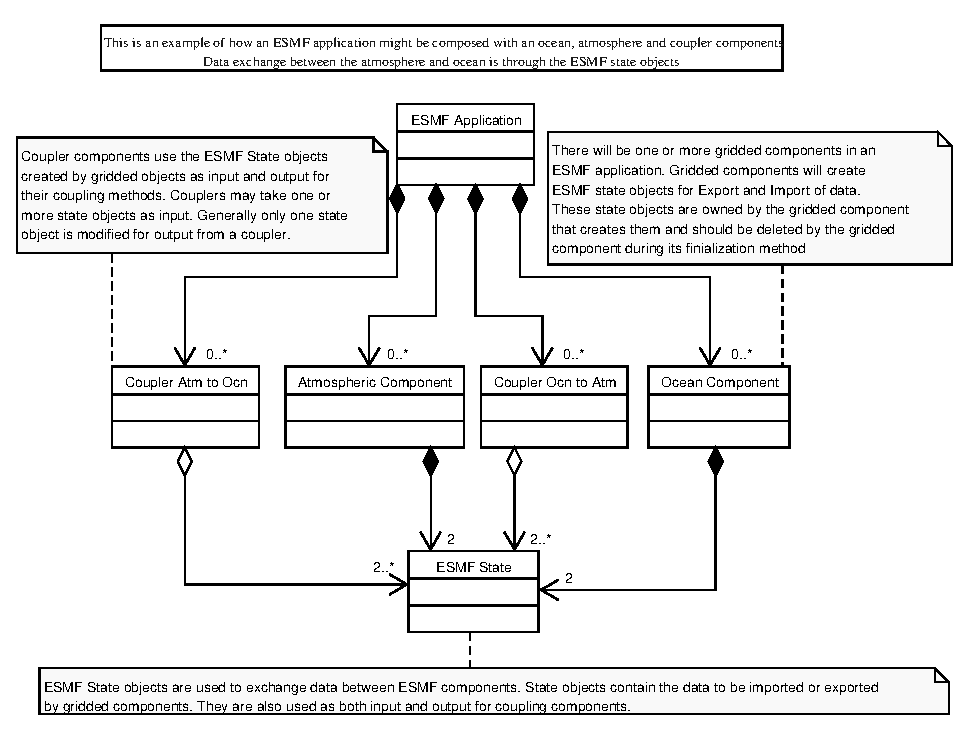
\includegraphics{ESMFSystemdiagram.eps}}
\end{figure}

\subsection{Transform (ESMF\_XForm)} 
A {\tt Transform} acts on a {\tt State} or other type of 
ESMF data.  It contains a function pointer to the transformation method
and may contain data necessary to perform the transform, frequency 
criteria and data
validation criteria.  It may relocate data, 
redistribute data, regrid data, change units, any combination of these,
or any other type of operation that the user desires.  









